\documentclass[letterpaper,12pt]{article}
\usepackage{tabularx,amsmath,boxedminipage,graphicx}
\usepackage[margin=1in,letterpaper]{geometry} % this shaves off default margins which are too big
\usepackage{cite}
\usepackage[final]{hyperref} % adds hyper links inside the generated pdf file
\usepackage{graphicx}
\usepackage{subfig}
\hypersetup{
	colorlinks=true,       % false: boxed links; true: colored links
	linkcolor=blue,          % color of internal links
	citecolor=blue,        % color of links to bibliography
	filecolor=magenta,      % color of file links
	urlcolor=blue         
}

\begin{document}

\title{ECE 232 Lab 3}
\author{Matthew Dombroski}
\date{March 21, 2016}
\maketitle

%  Abstract: A summary of the laboratory exercise, software that was implemented, data that was gathered, and
%  analysis that was completed.
%  • Code Implementation: A description of the code that was implemented to complete the lab. This is to be
%   written at the level of detail that qualitatively describes the files that were written and the purpose of the c++ functions that were implemented.
%  • Data and Data Analysis: The tables/plots of the data collected (as per the instructions of the  laboratory) and written descriptions of the observations.
%  • Laboratory Questions: Answers to the questions posted at the end of the laboratory.

 I affirm that I have not given or received any unauthorized help on this assignment,
and that all work is my own.
\begin{abstract}
For laboratory 3 a simplified beam model was implemented within the simulator written for the previous lab. In addition a GUI to visualize the position of the robot and feedback from the beams was built. Beam data with both the simulated robot and the Turtlebot with Kinect was collected and compared to see how the simulator matches up with the real world robot. 
\end{abstract}


\section{Code Implementation}
\subsection{GUI}
Within the file \texttt{gui.cpp} the functions \texttt{handle\_laserscan} and \texttt{handle\_odom} were written. The purpose of these function was to simply store the laser scan data and odometry data within class variables, which were declared in \texttt{gui.h}. This is then used within the \texttt{paintGL} function to draw the robot and beams in the correct location within a global system known by the simulator. Basic trigonometric calculations were used to compute the coordinates for drawn objects. 
\\\\ 
An additional line was added to the function \texttt{timer\_callback} to initiate a repaint of the screen. WIthout this line the screen would only redraw when clicked on or dragged. 

\subsection{Simulator}
The simulator replicated the physical layout given in the lab 3 instructions, with a 0.1m radius cone at 1m distance from the robot and a wall at 2m distance from the robot. The problem of replicating this physical layout was broken down into two main functions - \texttt{calcTrueDistance} and \texttt{calcNoisyDistance}. \texttt{calcTrueDistance} calculates the noise free beam ranges given a robot position and setup geometry. By sweeping over each angle for the beams the distance between wall or cone and the robot is computed. To calculate the distance to the wall simple trigonometry using parrallel lines is used. To calculate the distance between the robot and different point on the cone a more involved calculation is needed. First the angle between the oncoming beam and the radius of the cone intersecting the beam on the outer edge of the circle is computed using the equation:
$$b = asin\left(\frac{distance\_cone*sin(angle)}{cone\_radius}\right)$$
Next the angle between the radius and line segment connecting the robot's center point to the cone's center point is computed with the equation:
$$c = 180 - angle - b$$
Finally the distance to the edge of the cone is computed by the equation:
$$C = \frac{distance\_cone * sin(c)}{sin(b)}$$
The minimum and maximum angle for which the beam will intersect with the cone can be found by the formula:
$$angle\_min\_max = atan\left(\frac{radius\_cone}{distance\_cone}\right)$$ 
As the distance for each angle is computed the current beam angle is compared with the bound calculated by the equation above and if within those bounds the formulas for calculating the distance to the cone are used. Outside these bounds the normal equations for computing the distance to the wall are used. 
\\\\
After computing the true distances the noisy distances are calculated within \texttt{calcNoisyDistances}. To save a bit of computational power the true distances are only calculated once and afterward the noisy distances are calculated with every ROS update as the noisy distances are easier to compute. The noise for each beam is computed the same way the noise for the motion model was computed in the previous lab by summing 12 random values that are bounded by the variance of the measurement and then this value back to the true distance. 
\\\\
After all calculations are made the computed values are then published on the topic \texttt{\\scan} to be read by the GUI and any other nodes requiring the data. 

\subsection{Data Collection}
To write the beam data to a file the \texttt{ros\_subscriber} program written in lab 1 was modified. Another callback function \texttt{save\_scan} was added and all data contained in the \texttt{sensor\_msgs::LaserScan} message are written into a text file.

\section{Data and Analysis}
Figures 1 and 2 show the beam data collected. Figure 3 and 4 show screenshots of the GUI and drawing of the robot and beams.
\\\\
The most striking difference between the data collected was the noisiness of the sensor readings. The physical beam sensor has very little noise whereas the simulated beam model had a large proportion of noise. The mean distance readings from the simulator remained close the expected distance values. 
\\\\
In addition the cone appears to be much wider in the simulated beam model. The angular span of the lab cone is much smaller than the simulated cone. This could be from the fact that the cone from the lab had a smaller radius than the simulated cone. 
\\\\
Overall both the simulated and in lab beam data returned reasonable results. The sensors each gave a realistic and fairly accurate representation of what the world in front of the robot looked like.  
\begin{figure}
	\centering
	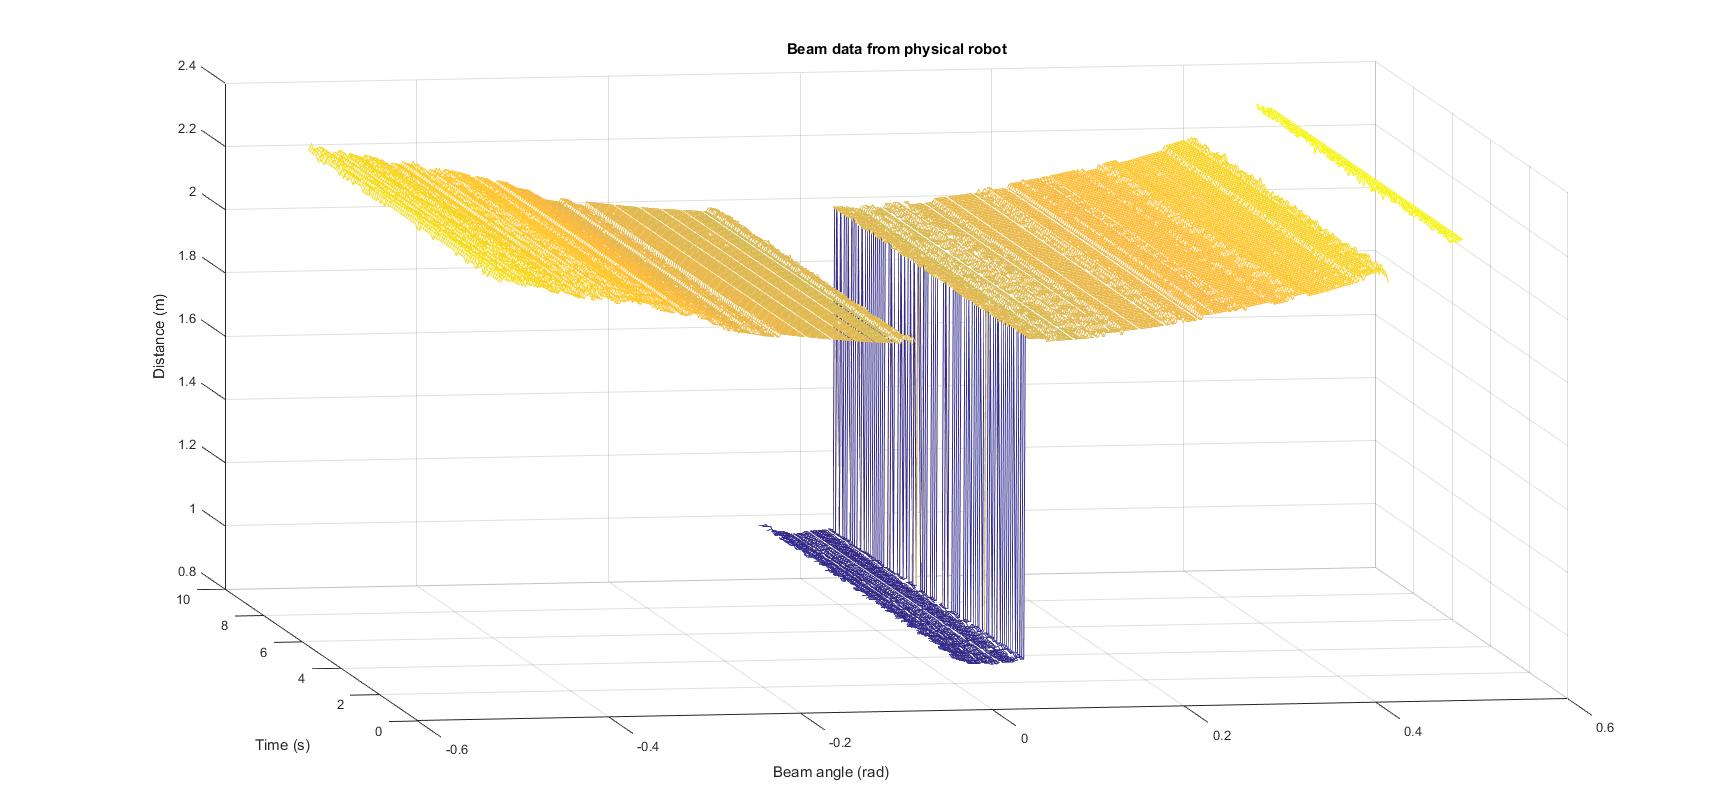
\includegraphics[width=.9\textwidth]{beamlab.jpg}\hfill
	\caption{Beam data from lab with a physical robot and beam sensor}
\end{figure}
\begin{figure}
	\centering
	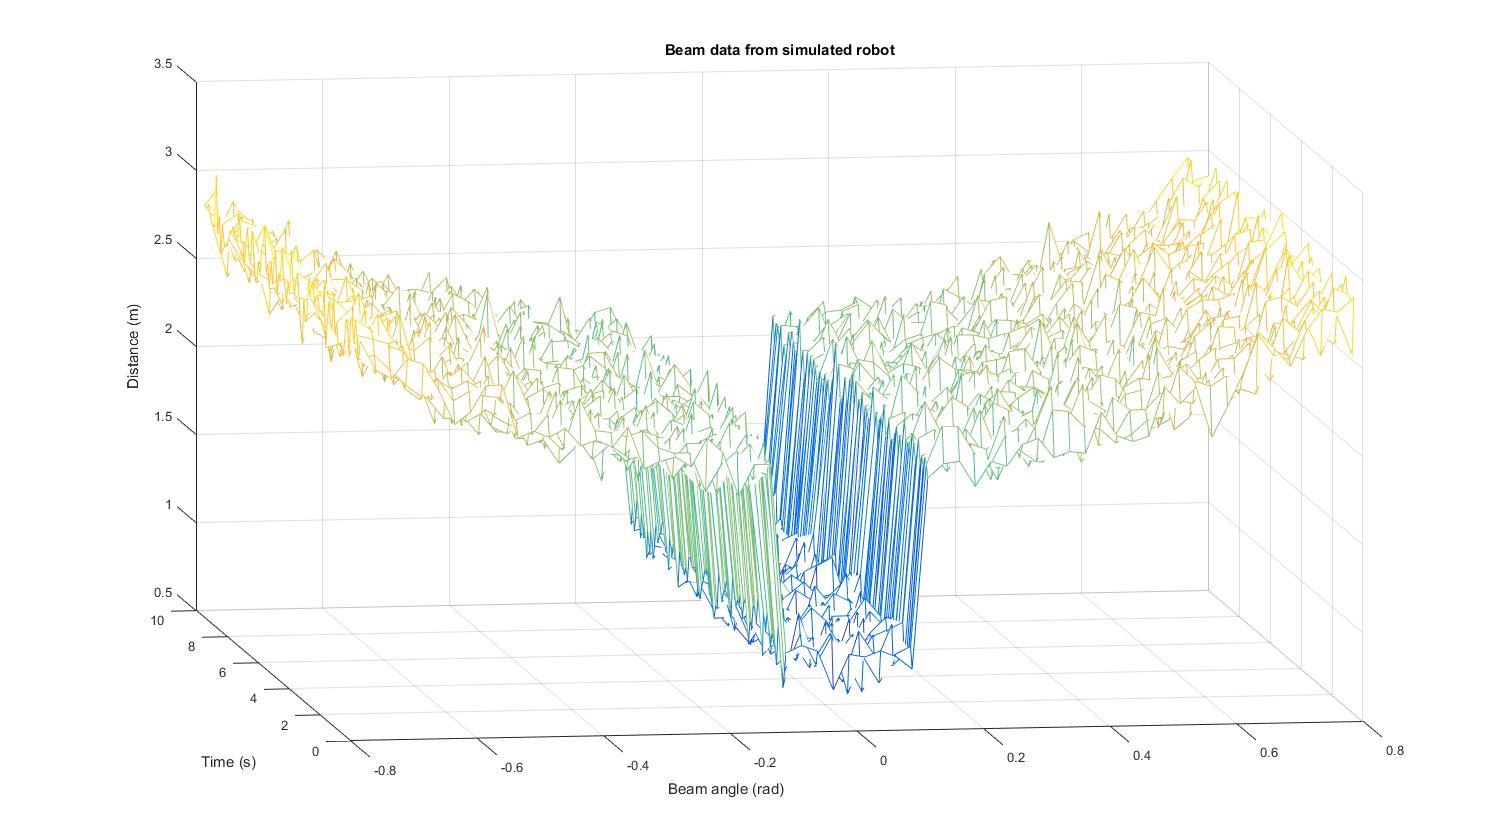
\includegraphics[width=.9\textwidth]{beamsim.jpg}\hfill
	\caption{Beam data from the simulator}
\end{figure}
\begin{figure}
	\centering
	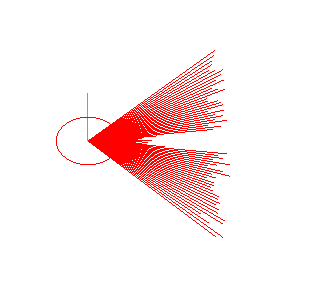
\includegraphics[width=.6\textwidth]{screenshotsim.jpg}\hfill
	\caption{Screenshot of beam model in the simulator}
\end{figure}
\begin{figure}
	\centering
	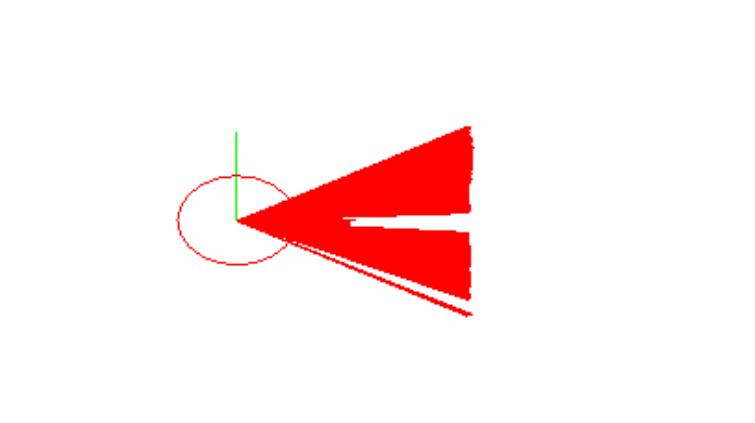
\includegraphics[width=.6\textwidth]{screenshotlab.jpg}\hfill
	\caption{Screenshot of the beam model from the lab}
\end{figure}


\section{Laboratory Questions}
Comparing the beam data between the simulator and physical robot two main difference are immediately noticeable. First the noise of the physical beam scan was much lower than that in the simulator. Where in the simulator there was upwards of 0.4m deviation the physical beam scan had a deviation of only a few hundredths of a meter. This discrepancy is more than likely the result of the fact that the variance of the physical scanner is lower than the variance used for the simulator. Another theory is that the function used to compress the 3D point cloud into planar ranges does some form of smoothing and filtering of the data, reducing the noise of the returned ranges. 
\\\\
Secondly it was observed that the width of the cone in the simulator was much wider than in the physical beam scans. Using data collected from lab it was found that the angular diameter of the cone was 0.0745 radians and the distance to the closest point of the cone was 0.937m. Using the formula relating angular diameter of an object to its radius the radius of the physical cone can be computed to be roughly equal to:
$$R=\sqrt{D^2-(Dcos(\frac{\alpha}{2})^2)}$$
$$R \approx 0.03m$$
Thus the radius of the cone in lab was approximately 30\% the radius of the cone in the simulated environment.   



%++++++++++++++++++++++++++++++++++++++++

% References section will be created automatically 
% with inclusion of "thebibliography" environment
% as it shown below. See text starting with line
% \begin{thebibliography}{99}




% There is a fancier and in long run more convinient way to do bibliography 
% with automatic inclusion of references from the bibliography database
% file. See usage of "bibtex" if you are interested in it.
% http://www.bibtex.org/
% but for know we will go with hand formated list.
% Note: with this approach it is YOUR responsibility to put them in order
% of appearance.
%\begin{thebibliography}{99}


%\bibitem{melissinos}
%A.~C. Melissinos and J. Napolitano, \textit{Experiments in Modern Physics},
%(Academic Press, New York, 2003).

%\bibitem{Cyr}
%N.\ Cyr, M.\ T$\hat{e}$tu, and M.\ Breton,
% "All-optical microwave frequency standard: a proposal,"
%IEEE Trans.\ Instrum.\ Meas.\ \textbf{42}, 640 (1993).

%\bibitem{Wiki} \emph{Expected value},  available at
%\texttt{http://en.wikipedia.org/wiki/Expected\_value}.

%\end{thebibliography}


\end{document}
